\documentclass[journal,11pt,onecolumn]{IEEEtran}
\usepackage{setspace}
\usepackage{gensymb}
\singlespacing
\usepackage[cmex10]{amsmath}
\usepackage{amsthm}
\usepackage{mathrsfs}
\usepackage{txfonts}
\usepackage{stfloats}
\usepackage{bm}
\usepackage{cite}
\usepackage{cases}
\usepackage{subfig}
\usepackage{longtable}
\usepackage{multirow}
\usepackage{enumitem}
\usepackage{mathtools}
\usepackage{tikz}
\usepackage{circuitikz}
\usepackage{verbatim}
\usepackage[breaklinks=true]{hyperref}
\usepackage{tkz-euclide} % loads  TikZ and tkz-base
\usepackage{listings}
\usepackage{color}    
\usepackage{array}    
\usepackage{longtable}
\usepackage{calc}     
\usepackage{multirow} 
\usepackage{hhline}   
\usepackage{ifthen}   
\usepackage{lscape}     
\usepackage{chngcntr}
\usepackage{float}
\DeclareMathOperator*{\Res}{Res}
\renewcommand\thesection{\arabic{section}}
\renewcommand\thesubsection{\thesection.\arabic{subsection}}
\renewcommand\thesubsubsection{\thesubsection.\arabic{subsubsection}}

\renewcommand\thesectiondis{\arabic{section}}
\renewcommand\thesubsectiondis{\thesectiondis.\arabic{subsection}}
\renewcommand\thesubsubsectiondis{\thesubsectiondis.\arabic{subsubsection}}
\renewcommand\thetable{\arabic{table}}
% correct bad hyphenation here
\hyphenation{op-tical net-works semi-conduc-tor}
\def\inputGnumericTable{}                                 %%

\lstset{
%language=C,
frame=single, 
breaklines=true,
columns=fullflexible
}
%\lstset{
%language=tex,
%frame=single, 
%breaklines=true
%}
\providecommand{\pr}[1]{\ensuremath{\Pr\left(#1\right)}}
\providecommand{\prt}[2]{\ensuremath{p_{#1}^{\left(#2\right)} }}        % own macro for this question
\providecommand{\qfunc}[1]{\ensuremath{Q\left(#1\right)}}
\providecommand{\sbrak}[1]{\ensuremath{{}\left[#1\right]}}
\providecommand{\lsbrak}[1]{\ensuremath{{}\left[#1\right.}}
\providecommand{\rsbrak}[1]{\ensuremath{{}\left.#1\right]}}
\providecommand{\brak}[1]{\ensuremath{\left(#1\right)}}
\providecommand{\lbrak}[1]{\ensuremath{\left(#1\right.}}
\providecommand{\rbrak}[1]{\ensuremath{\left.#1\right)}}
\providecommand{\cbrak}[1]{\ensuremath{\left\{#1\right\}}}
\providecommand{\lcbrak}[1]{\ensuremath{\left\{#1\right.}}
\providecommand{\rcbrak}[1]{\ensuremath{\left.#1\right\}}}
\newcommand{\sgn}{\mathop{\mathrm{sgn}}}
\providecommand{\abs}[1]{\left\vert#1\right\vert}
\providecommand{\res}[1]{\Res\displaylimits_{#1}} 
\providecommand{\norm}[1]{\left\lVert#1\right\rVert}
%\providecommand{\norm}[1]{\lVert#1\rVert}
\providecommand{\mtx}[1]{\mathbf{#1}}
\providecommand{\mean}[1]{E\left[ #1 \right]}
\providecommand{\cond}[2]{#1\middle|#2}
\providecommand{\fourier}{\overset{\mathcal{F}}{ \rightleftharpoons}}
%\providecommand{\hilbert}{\overset{\mathcal{H}}{ \rightleftharpoons}}
%\providecommand{\system}{\overset{\mathcal{H}}{ \longleftrightarrow}}
	%\newcommand{\solution}[2]{\textbf{Solution:}{#1}}
\newcommand{\solution}{\noindent \textbf{Solution: }}
\newcommand{\cosec}{\,\text{cosec}\,}
\providecommand{\dec}[2]{\ensuremath{\overset{#1}{\underset{#2}{\gtrless}}}}
\newcommand{\myvec}[1]{\ensuremath{\begin{pmatrix}#1\end{pmatrix}}}
\newcommand{\mydet}[1]{\ensuremath{\begin{vmatrix}#1\end{vmatrix}}}
\providecommand{\rank}{\text{rank}}
\providecommand{\pr}[1]{\ensuremath{\Pr\left(#1\right)}}
\providecommand{\qfunc}[1]{\ensuremath{Q\left(#1\right)}}
	\newcommand*{\permcomb}[4][0mu]{{{}^{#3}\mkern#1#2_{#4}}}
\newcommand*{\perm}[1][-3mu]{\permcomb[#1]{P}}
\newcommand*{\comb}[1][-1mu]{\permcomb[#1]{C}}
\providecommand{\qfunc}[1]{\ensuremath{Q\left(#1\right)}}
\providecommand{\gauss}[2]{\mathcal{N}\ensuremath{\left(#1,#2\right)}}
\providecommand{\diff}[2]{\ensuremath{\frac{d{#1}}{d{#2}}}}
\providecommand{\myceil}[1]{\left \lceil #1 \right \rceil }
\newcommand\figref{Fig.~\ref}
\newcommand\tabref{Table~\ref}
\newcommand{\sinc}{\,\text{sinc}\,}
\newcommand{\rect}{\,\text{rect}\,}
\title{Assignment}
\author{Barath surya M | EE22BTECH11014}
\begin{document}
\newtheorem{theorem}{Theorem}[section]
\newtheorem{problem}{Problem}
\newtheorem{proposition}{Proposition}[section]
\newtheorem{lemma}{Lemma}[section]
\newtheorem{corollary}[theorem]{Corollary}
\newtheorem{example}{Example}[section]
\newtheorem{definition}[problem]{Definition}
\newcommand{\BEQA}{\begin{eqnarray}}
\newcommand{\EEQA}{\end{eqnarray}}
\newcommand{\define}{\stackrel{\triangle}{=}}
\bibliographystyle{IEEEtran}
\providecommand{\mbf}{\mathbf}
\providecommand{\pr}[1]{\ensuremath{\Pr\left(#1\right)}}
\providecommand{\qfunc}[1]{\ensuremath{Q\left(#1\right)}}
\providecommand{\sbrak}[1]{\ensuremath{{}\left[#1\right]}}
\providecommand{\lsbrak}[1]{\ensuremath{{}\left[#1\right.}}
\providecommand{\rsbrak}[1]{\ensuremath{{}\left.#1\right]}}
\providecommand{\brak}[1]{\ensuremath{\left(#1\right)}}
\providecommand{\lbrak}[1]{\ensuremath{\left(#1\right.}}
\providecommand{\rbrak}[1]{\ensuremath{\left.#1\right)}}
\providecommand{\cbrak}[1]{\ensuremath{\left\{#1\right\}}}
\providecommand{\lcbrak}[1]{\ensuremath{\left\{#1\right.}}
\providecommand{\rcbrak}[1]{\ensuremath{\left.#1\right\}}}
\theoremstyle{remark}
\newtheorem{rem}{Remark}
\providecommand{\abs}[1]{\left\vert#1\right\vert}
\providecommand{\res}[1]{\Res\displaylimits_{#1}} 
\providecommand{\norm}[1]{\left\lVert#1\right\rVert}
\providecommand{\mtx}[1]{\mathbf{#1}}
\providecommand{\mean}[1]{E\left[ #1 \right]}
\providecommand{\fourier}{\overset{\mathcal{F}}{ \rightleftharpoons}}
\providecommand{\system}[1]{\overset{\mathcal{#1}}{ \longleftrightarrow}}
\providecommand{\dec}[2]{\ensuremath{\overset{#1}{\underset{#2}{\gtrless}}}}
\let\vec\mathbf
\def\putbox#1#2#3{\makebox[0in][l]{\makebox[#1][l]{}\raisebox{\baselineskip}[0in][0in]{\raisebox{#2}[0in][0in]{#3}}}}
     \def\rightbox#1{\makebox[0in][r]{#1}}
     \def\centbox#1{\makebox[0in]{#1}}
     \def\topbox#1{\raisebox{-\baselineskip}[0in][0in]{#1}}
     \def\midbox#1{\raisebox{-0.5\baselineskip}[0in][0in]{#1}}
\maketitle
Question 9.3.3
Five cards are drawn successively with replacement from well shuffled deck of 52 cards, what is the probability that
\begin{enumerate}
	\item all the five cards are spades?
	\item only 3 cards are spades
	\item None is a spade
\end{enumerate}
\solution\\
\textbf{Binomial}\\
Let X be a binomial random variable representing the number of spade cards among the five cards and with the parameters n and p as,
\begin{align}
	n&=5\\
	p&=\frac{13}{52}\\
	&=0.25
\end{align}
PMF of the distribution is,
\begin{align}
	\pr{X=k}&=\comb{n}{k}p^k\brak{1-p}^{n-k}
\end{align}
\begin{enumerate}
	\item
	\begin{align}
	k&=5\\
	\implies \pr{X=5}&=\comb{5}{5}\brak{0.25}^5\brak{0.75}^0\\
	&=0.0009765625
\end{align}
	\item
	\begin{align}
	k&=3\\
	\pr{X=3}&=\comb{5}{3}\brak{0.25}^3\brak{0.75}^2\\
	&=0.087890625
\end{align}
	\item
	\begin{align}
	k&=0\\
	\pr{X=0}&=\comb{5}{0}\brak{0.25}^0\brak{0.75}^5\\
	&=0.2373046875
\end{align}
\end{enumerate}
\textbf{Gaussian}\\
\begin{align}
	X &\sim Bin\brak{n,p}\\
	&\sim Bin\brak{5,0.25}
\end{align}
Mean and varience of X are
\begin{align}
	\mu_X&=np\\
	&=1.25\\
	\sigma^2_X&=np\brak{1-q}\\
	&=0.9375
\end{align}
Let,Z be a rondom variable with mean $\mu_Z = 0$ and $\sigma_Z=1$, such that,
\begin{align}
	Z&=\frac{X- \mu_X}{\sigma_X}
\end{align}
Z caoverges to normal distribution for large value of n
\begin{align}
	f\brak{x}&=\frac{1}{\sqrt{2\pi}}e^{-\frac{x^2}{2}}
\end{align}
And the Q funtion is 
\begin{align}
	\qfunc{x}&=\pr{Z >x}
\end{align}
\begin{enumerate}
	\item 
	\begin{align}
		X&=5
	\end{align}
	\begin{align}
	\pr{Z=\frac{X-\mu_X}{\sigma_X}} &\approx \pr{\frac{X+0.5-\mu_X}{\sigma_X} < Z < \frac{X-0.5-\mu_X}{\sigma_X}}\\
	&\approx \pr{Z<\frac{X+0.5-\mu_X}{\sigma_X}} - \pr{Z<\frac{X-0.5-\mu_X}{\sigma_X}}\\
	&\approx \pr{Z>\frac{X-0.5-\mu_X}{\sigma_X}} - \pr{Z>\frac{X+0.5-\mu_X}{\sigma_X}}\\
	&\approx \qfunc{\frac{X-0.5-\mu_X}{\sigma_X}} - \qfunc{\frac{X+0.5-\mu_X}{\sigma_X}}\\
	&\approx \qfunc{3.356} - \qfunc{4.389}\\
	&\approx 0.0003888
	\end{align}
	\item 
	\begin{align}
		X&=3
	\end{align}
	\begin{align}
	\pr{Z=\frac{X-\mu_X}{\sigma_X}} &\approx \pr{\frac{X+0.5-\mu_X}{\sigma_X} < Z < \frac{X-0.5-\mu_X}{\sigma_X}}\\
	&\approx \pr{Z<\frac{X+0.5-\mu_X}{\sigma_X}} - \pr{Z<\frac{X-0.5-\mu_X}{\sigma_X}}\\
	&\approx \pr{Z>\frac{X-0.5-\mu_X}{\sigma_X}} - \pr{Z>\frac{X+0.5-\mu_X}{\sigma_X}}\\
	&\approx \qfunc{\frac{X-0.5-\mu_X}{\sigma_X}} - \qfunc{\frac{X+0.5-\mu_X}{\sigma_X}}\\
	&\approx \qfunc{1.2909} - \qfunc{2.3237}\\
	&\approx 0.08828
	\end{align}
	\item 
	\begin{align}
		X&=0
	\end{align}
	\begin{align}
	\pr{Z=\frac{X-\mu_X}{\sigma_X}} &\approx \pr{\frac{X+0.5-\mu_X}{\sigma_X} < Z < \frac{X-0.5-\mu_X}{\sigma_X}}\\
	&\approx \pr{Z<\frac{X+0.5-\mu_X}{\sigma_X}} - \pr{Z<\frac{X-0.5-\mu_X}{\sigma_X}}\\
	&\approx \pr{Z>\frac{X-0.5-\mu_X}{\sigma_X}} - \pr{Z>\frac{X+0.5-\mu_X}{\sigma_X}}\\
	&\approx \qfunc{\frac{X-0.5-\mu_X}{\sigma_X}} - \qfunc{\frac{X+0.5-\mu_X}{\sigma_X}}\\
	&\approx \qfunc{-1.8073} - \qfunc{-0.7745}\\
	&\approx 0.1839
	\end{align}
\end{enumerate}

\begin{figure}[ht!]
	\centering
	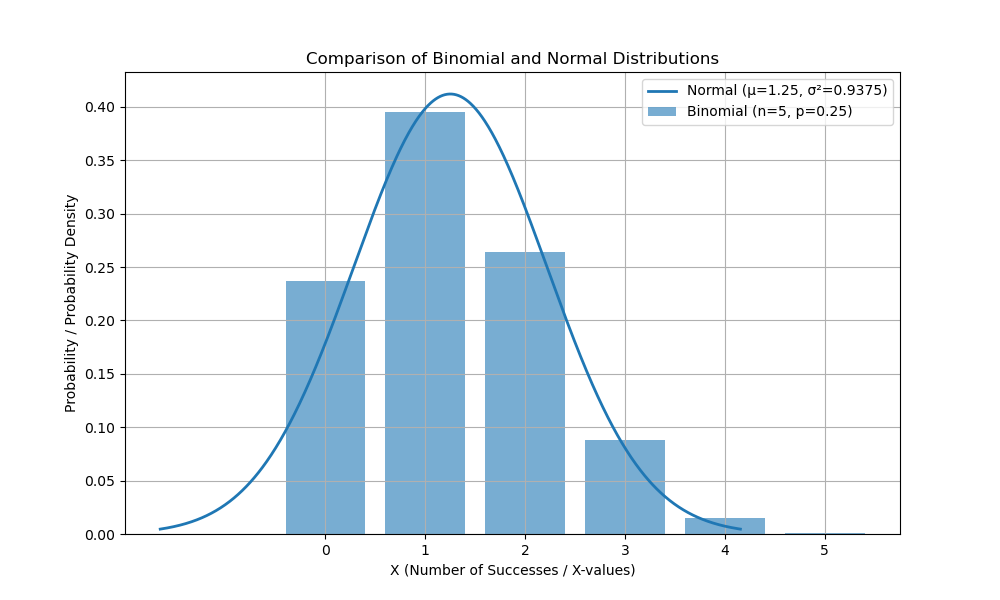
\includegraphics[width=\columnwidth]{figs/fig.png}
	\caption{Binomial and gaussian distribution}
\end{figure}
\end{document}
